\begin{pastexam}[label={px:ntust-108-ice-06}]{臺科大資工所 108 學年度 第 6 題}
（問答）

Please show the minimum spanning tree of the graph in Fig. 2. (8\%)

\begin{center}
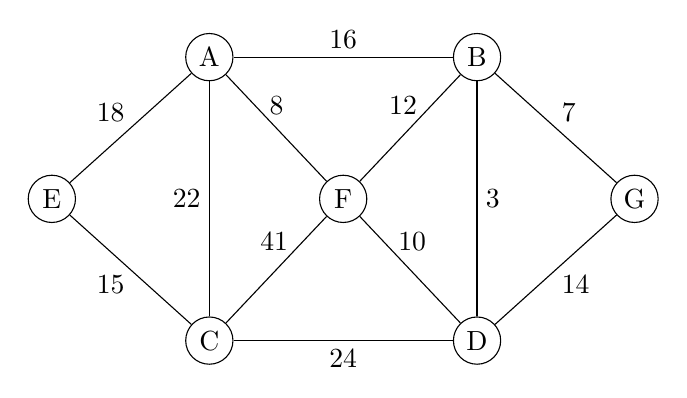
\begin{tikzpicture}[v/.style={circle,draw,inner sep=1.5pt,minimum size=6mm},w/.style={inner sep=1pt}]
\node[v] (A) at (2,3.6) {A};
\node[v] (B) at (5.4,3.6) {B};
\node[v] (E) at (0,1.8) {E};
\node[v] (F) at (3.7,1.8) {F};
\node[v] (G) at (7.4,1.8) {G};
\node[v] (C) at (2,0) {C};
\node[v] (D) at (5.4,0) {D};
\draw (A) -- node[w,above=2pt] {16} (B);
\draw (A) -- node[w,above left=1pt] {18} (E);
\draw (A) -- node[w,left=2pt] {22} (C);
\draw (A) -- node[w,pos=0.4,above right=0pt] {8} (F);
\draw (B) -- node[w,pos=0.4,above left=0pt] {12} (F);
\draw (B) -- node[w,right=2pt] {3} (D);
\draw (B) -- node[w,above right=1pt] {7} (G);
\draw (E) -- node[w,below left=1pt] {15} (C);
\draw (F) -- node[w,pos=0.35,above left=0pt] {41} (C);
\draw (F) -- node[w,pos=0.35,above right=0pt] {10} (D);
\draw (C) -- node[w,below=2pt] {24} (D);
\draw (D) -- node[w,below right=1pt] {14} (G);
\end{tikzpicture}

Fig. 2
\end{center}
\end{pastexam}

\begin{pastsoln}
答案：最小生成樹的邊是 $BD(3)$、$BG(7)$、$AF(8)$、$FD(10)$、$EC(15)$、$AE(18)$，總權重 $61$。

用 Kruskal 演算法（資結書第~24.2~節）：邊依權重由小到大檢查，兩端已經連通（加了會成環）就跳過，
否則加入。 圖有 $7$ 個頂點，加到 $6$ 條邊就完成。
\begin{center}
\small
\begin{tabular}{cccl}
\toprule
權重 & 邊 & 結果 & 加入後的連通塊（只列兩個點以上的） \\
\midrule
$3$ & $BD$ & 加入 & $\{B, D\}$ \\
$7$ & $BG$ & 加入 & $\{B, D, G\}$ \\
$8$ & $AF$ & 加入 & $\{B, D, G\}$、$\{A, F\}$ \\
$10$ & $FD$ & 加入 & $\{A, B, D, F, G\}$ \\
$12$ & $BF$ & 跳過 & $B$、$F$ 已連通（$B$--$D$--$F$） \\
$14$ & $DG$ & 跳過 & $D$、$G$ 已連通（$D$--$B$--$G$） \\
$15$ & $EC$ & 加入 & $\{A, B, D, F, G\}$、$\{C, E\}$ \\
$16$ & $AB$ & 跳過 & $A$、$B$ 已連通（$A$--$F$--$D$--$B$） \\
$18$ & $AE$ & 加入 & 全部 $7$ 個頂點，共 $6$ 條邊，結束 \\
\bottomrule
\end{tabular}
\end{center}
總權重 $3 + 7 + 8 + 10 + 15 + 18 = 61$。
\begin{center}
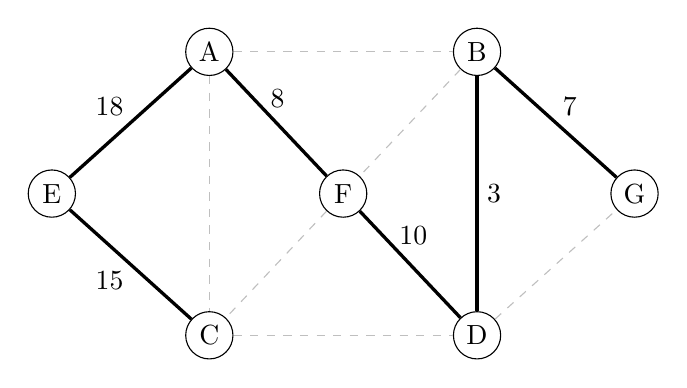
\begin{tikzpicture}[v/.style={circle,draw,inner sep=1.5pt,minimum size=6mm},w/.style={inner sep=1pt},
  t/.style={very thick},o/.style={draw=black!25,dashed}]
\node[v] (A) at (2,3.6) {A};
\node[v] (B) at (5.4,3.6) {B};
\node[v] (E) at (0,1.8) {E};
\node[v] (F) at (3.7,1.8) {F};
\node[v] (G) at (7.4,1.8) {G};
\node[v] (C) at (2,0) {C};
\node[v] (D) at (5.4,0) {D};
\draw[o] (A) -- (B);
\draw[o] (A) -- (C);
\draw[o] (B) -- (F);
\draw[o] (F) -- (C);
\draw[o] (C) -- (D);
\draw[o] (D) -- (G);
\draw[t] (A) -- node[w,above left=1pt] {18} (E);
\draw[t] (A) -- node[w,pos=0.4,above right=0pt] {8} (F);
\draw[t] (B) -- node[w,right=2pt] {3} (D);
\draw[t] (B) -- node[w,above right=1pt] {7} (G);
\draw[t] (E) -- node[w,below left=1pt] {15} (C);
\draw[t] (F) -- node[w,pos=0.35,above right=0pt] {10} (D);
\end{tikzpicture}
\end{center}
粗線是最小生成樹，虛線是沒選的邊。

所有邊的權重都不相同，所以最小生成樹只有這一棵（資結書定理~24.4）。 用 Prim 演算法（資結書
第~24.3~節）從 $A$ 出發會依序加入 $AF(8)$、$FD(10)$、$DB(3)$、$BG(7)$、$AE(18)$、$EC(15)$，得到同一棵樹。
\end{pastsoln}
